\chapter{实验环境搭建}

\section{仿真环境配置}

\subsection{Carla 仿真平台}


Carla 是个开源的自动驾驶模拟平台,能提供超真实的交通场景和车辆动力学模型。在这项研究中,选择用 Carla 的 Town10 模拟场景做实验。Town10 这个场景有多个十字路口、各种车道,还有超多的交通元素,能模拟现实交通里的各种复杂情况,是测试多目标跟踪算法的好基础。

版本选择:本次设计中安装的是 Carla 0.9.15 版本,这个版本在功能和稳定性上完全能满足咱们的实验需求。

场景加载:通过 Carla 的客户端程序把 Town10 场景加载出来,得确保场景里的道路、建筑、交通标志等元素都能正确显示。

传感器配置:在 Carla 里给车辆配上各种传感器,像 RGB 相机、深度相机和激光雷达之类的。RGB 相机是负责拍交通场景的视觉图像的,深度相机和激光雷达则是用来测目标物体的距离的。这些传感器的数据都会输给多目标跟踪算法。根据实验需要,合理设置传感器的参数,比如分辨率、帧率、视角这些,好拿到高质量的模拟数据。



\subsection{Pycharm环境配置}
根据课题要求,本项目进一步搭建了与 Town10 仿真场景相关的交通数字孪生环境,用于获取目标的真实跟踪轨迹(Ground Truth)以及优化检测跟踪模型。

环境搭建:首先,根据项目与课题的要求,创建 Python 3.8 的虚拟环境,并安装如表~\ref{tab:full-dependencies} 所示的关键依赖包

\begin{table}[htbp]
	\centering
	\caption{Python 虚拟环境完整依赖清单}
	\label{tab:full-dependencies}
	\begin{tabular}{lll}
		\hline
		\textbf{类别} & \textbf{包名称} & \textbf{版本} \\ 
		\hline
		\multirow{8}{*}{核心依赖}
		& numpy & 1.24.4 \\
		& scipy & 1.10.1 \\
		& protobuf & $\geq$3.6 \\
		& future & $\geq$0.16.0 \\
		& psutil & 6.1.0 \\
		& opencv-python & 4.10.0.84 \\
		& pillow & 10.4.0 \\
		& open3d & 0.18.0 \\
		
		\hline
		\multirow{6}{*}{仿真交互}
		& carla & 0.9.15 \\
		& pygame & $\geq$1.9.4 \\
		& pywin32 & 308 \\
		& configargparse & 1.7 \\
		& retrying & 1.3.4 \\
		& tenacity & 9.0.0 \\
		
		\hline
		\multirow{7}{*}{数据处理}
		& pandas & 2.0.3 \\
		& python-dateutil & 2.9.0.post0 \\
		& pyparsing & 3.1.4 \\
		& contourpy & 1.1.1 \\
		& cycler & 0.12.1 \\
		& fonttools & 4.55.1 \\
		& packaging & 24.2 \\
		
		\hline
		\multirow{6}{*}{可视化}
		& matplotlib & 3.7.5 \\
		& plotly & 5.24.1 \\
		& dash & 2.18.2 \\
		& dash-core-components & 2.0.0 \\
		& dash-html-components & 2.0.0 \\
		& dash-table & 5.0.0 \\
		
		\hline
		\multirow{8}{*}{开发工具}
		& ipython & 8.12.3 \\
		& jedi & 0.19.2 \\
		& traitlets & 5.14.3 \\
		& prompt-toolkit & 3.0.48 \\
		& pygments & 2.18.0 \\
		& wcwidth & 0.2.13 \\
		& platformdirs & 4.3.6 \\
		& executing & 2.1.0 \\
		
		\hline
		\multirow{6}{*}{Web框架}
		& flask & 3.0.3 \\
		& werkzeug & 3.0.6 \\
		& jinja2 & 3.1.5 \\
		& itsdangerous & 2.2.0 \\
		& click & 8.1.8 \\
		& blinker & 1.8.2 \\
		
		
		
		\hline
	\end{tabular}
\end{table}

航点控制与轨迹平滑:利用项目中的航点控制模块,获取车辆在 Town10 场景中的运行航点。通过轨迹平滑算法生成连续轨迹,主要依赖 scipy 的信号处理模块和 numpy 的数值计算功能,相关算法实现基于表~\ref{tab:full-dependencies} 中的科学计算库。

PID 控制器:采用 PID 控制算法对车辆进行控制,其核心实现依赖 numpy 进行矩阵运算,同时利用 matplotlib 进行控制过程可视化。表~\ref{tab:full-dependencies} 中列出的实时数据可视化工具 dash 用于构建控制参数调试界面。

\subsection{Matlab环境配置}

版本:Matlab2024b,如图\ref{fig:p7}matlab环境。


\begin{figure}[htbp] % 可以是h(here),t(top),b(bottom),p(page of floats)
	\centering
	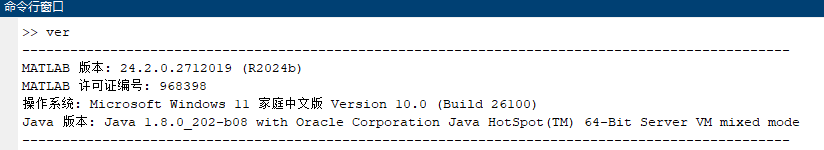
\includegraphics[width=1\textwidth]{p7} % 假设图片文件名为car.pdf或car.png等,位于当前工作目录
	\caption{matlab环境} % 图片标题
	\label{fig:p7} % 用于引用的标签
\end{figure}


MATLAB 算法开发平台,它的图像处理工具箱和计算机视觉工具箱为多目标跟踪算法的开发提供了各种好用的工具和函数。用这些工具箱,能快速把各种多目标跟踪算法实现出来并测试,比如卡尔曼滤波、联合概率数据关联滤波这些经典算法,还有结合深度学习的目标检测和跟踪算法。在 MATLAB 里实现这些算法后,可以方便地评估算法性能,调调参数,再和现有的 Baseline 算法对比分析。

在实验中,收集的数据又多又复杂,不过 MATLAB 的数据处理工具箱很给力,像信号处理工具箱和统计与机器学习工具箱如图\ref{fig:p8},能高效地对交通场景中的传感器数据进行预处理、特征提取和统计分析。比如,可以用这些工具箱对从 Carla 仿真平台获取的车辆轨迹数据进行滤波,去除噪声,提取关键特征点,还能对多目标的运动模式进行建模和分析。



\begin{figure}[htbp] % 可以是h(here),t(top),b(bottom),p(page of floats)
	\centering
	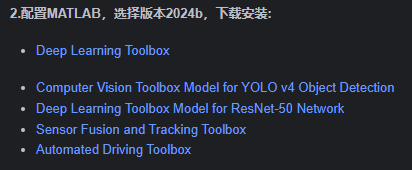
\includegraphics[width=1\textwidth]{p8} % 假设图片文件名为car.pdf或car.png等,位于当前工作目录
	\caption{matlab配置} % 图片标题
	\label{fig:p8} % 用于引用的标签
\end{figure}






\section{实验设备与软件工具}

\subsection{硬件设备}

设备名称:DESKTOP-H2JCRHP

处理器:AMD Ryzen 7 5800H with Radeon Graphics            3.20 GHz

机带:RAM	16.0 GB (15.4 GB 可用)

设备 ID:9FF8ABE5-216E-4C15-B738-D4364271428F

产品 ID:00326-40000-00000-AAOEM

系统类型:64 位操作系统, 基于 x64 的处理器

GPU:NVIDlA GeForce RTX 3060 Laptop GPU 与 Radeon(TM) Graphics

内存:1.32TB

该硬件配置能让 Carla 仿真平台跑起来,同时保障多目标跟踪算法的高效训练和测试。还装了大容量固态硬盘(SSD),能存 Carla 的场景数据、传感器数据以及实验中产生的大量模型和结果数据,这样数据读写快,存储也安全。


\subsection{软件工具}

拥有全面的软件工具才能让设计顺利地进行,如图\ref{fig:p31}是本次设计所需要的软件工具。

操作系统:Windows 11

本研究的编程语言主要选 Python,用它来开发算法和写实验脚本。开发工具是 PyCharm,它集成了代码编辑、调试、版本控制等功能,方便又高效。另外,装好了 carla、NumPy、SciPy、OpenCV 等常用 Python 库,这些库在数据处理、图像处理和数学计算方面都很好用。

深度学习框架选的是 PyTorch,这框架模型构建灵活,还有强大的自动微分功能,特别适合实现和优化多目标跟踪模型。同时,安装了 torchvision 等相关依赖包,为模型的训练和测试提供了坚实的支持。
数据库管理系统用的是 MySQL,用它搭建了路口车辆航点到 Carla 坐标映射的数据库。创建了相应的数据表,存储路口、车道、方向等信息以及对应的 Carla 场景中道路终点坐标位置(x, y, z 和 yaw),为路口导航和目标跟踪提供了可靠的数据支持。

数据预处理和格式转换这块,本此设计选择的是Matlab2024b 工具。它能做多模态数据处理、快速验证算法和量化评估性能,还配备了 Computer Vision Toolbox、Sensor Fusion and Tracking Toolbox 等丰富的工具箱,大大提高了开发效率。在轨迹优化、跨传感器融合和可视化方面,它提供了高效的解决方案,对智慧交通场景下多目标跟踪算法的研究和实际应用都有很大的帮助。




\begin{figure}[htbp] % 可以是h(here),t(top),b(bottom),p(page of floats)
	\centering
	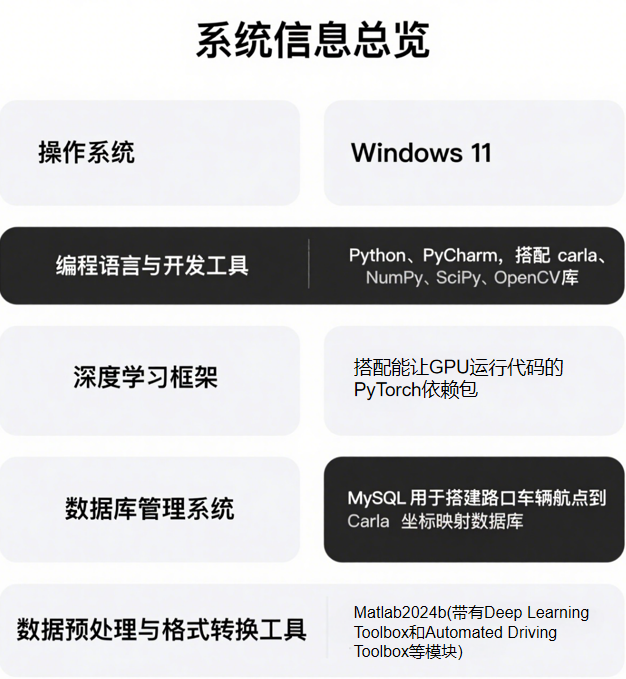
\includegraphics[width=0.75\textwidth]{p31} % 假设图片文件名为car.pdf或car.png等,位于当前工作目录
	\caption{软件工具} % 图片标题
	\label{fig:p31} % 用于引用的标签
\end{figure}









